\documentclass[11pt,twoside]{book}
\usepackage[mono=false]{libertine} % new linux font, ignore mono
\usepackage{luatex85}

\usepackage{amsmath,amsthm,amssymb,mathrsfs,amsfonts,dsfont}
\usepackage{epsfig,graphicx}
\usepackage{tabularx}
\usepackage{blkarray}
\usepackage{slashed}
\usepackage{color}
\usepackage{listings}
\lstset{
    language=bash,
    basicstyle=\ttfamily,
    breaklines=true,
    showstringspaces=false,
    commentstyle=\color{green!40!black},
    keywordstyle=\color{blue},
    stringstyle=\color{orange}
}
\usepackage{caption}
\usepackage{lipsum} % provides dummy text for testing
\usepackage[toc,title,titletoc,header]{appendix}
\usepackage{minitoc}
\usepackage{multicol} % two-col ToC
\usepackage{bm}
\usepackage{imakeidx} % before hyperref
\usepackage{hyperref}
\hypersetup{
    colorlinks=true,
    citecolor=magenta,
    linkcolor=black,
    filecolor=green,      
    urlcolor=cyan,
}
\usepackage[capitalise]{cleveref}
\usepackage{subcaption}
\usepackage{enumitem}
\usepackage{mathtools}
\usepackage{physics}
\usepackage[linesnumbered,ruled,vlined,algosection]{algorithm2e}
\SetCommentSty{textsf}
\usepackage{epigraph}
\epigraphwidth=1.0\linewidth
\epigraphrule=0pt

% adjust margin
\usepackage[margin=2.3cm]{geometry}
\headheight13.6pt

\usepackage{fancyhdr}
\pagestyle{fancy} % enable fancy page style
\renewcommand{\headrulewidth}{0.0pt} % comment if you want the rule
\fancyhf{} % clear header and footer
\fancyhead[lo,le]{\leftmark}
\fancyhead[re,ro]{\rightmark}
\fancyfoot[CE,CO]{\hyperref[toc-contents]{\thepage}}

\makeatletter
\def\chaptermark#1{\markboth{\protect\hyper@linkstart{link}{\@currentHref}{Chapter \thechapter ~ #1}\protect\hyper@linkend}{}}
\def\sectionmark#1{\markright{\protect\hyper@linkstart{link}{\@currentHref}{\thesection ~ #1}\protect\hyper@linkend}}
\makeatother

\usepackage[doi=false,url=false,isbn=false,style=alphabetic,backend=biber,backref=true]{biblatex}
\addbibresource{bib.bib}

\newbibmacro{string+doiurlisbn}[1]{%
  \iffieldundef{doi}{%
    \iffieldundef{url}{%
      \iffieldundef{isbn}{%
        \iffieldundef{issn}{%
          #1%
        }{%
          \href{http://books.google.com/books?vid=ISSN\thefield{issn}}{#1}%
        }%
      }{%
        \href{http://books.google.com/books?vid=ISBN\thefield{isbn}}{#1}%
      }%
    }{%
      \href{\thefield{url}}{#1}%
    }%
  }{%
    \href{http://dx.doi.org/\thefield{doi}}{#1}%
  }%
}

\DeclareFieldFormat[article,incollection,inproceedings,book,misc]{title}{\usebibmacro{string+doiurlisbn}{\mkbibemph{#1}}}
\DeclareFieldFormat{journaltitle}{#1\isdot}
\DeclareFieldFormat{booktitle}{#1\isdot}
\renewbibmacro{in:}{}
\DeclareSourcemap{
    \maps[datatype=bibtex]{
      \map{
        \step[fieldsource=video]
        \step[fieldset=usera,origfieldval]
    }
  }
}
\DeclareFieldFormat{usera}{\href{#1}{\textsc{Online video}}}
\AtEveryBibitem{
    \csappto{blx@bbx@\thefield{entrytype}}{% put at end of entry
        \iffieldundef{usera}{}{\space \printfield{usera}}
    }
}



% !TEX root = ./notes_template.tex

%%%%%%%%%%%%%%%%%%%%%%%%%%%%%%%%%%%%
%%%%%%%%%%%%%%%%%%%%%%%%%%%%%%%%%%%%
% math
\let\iff\relax
\newcommand{\iff}{\text{ iff }}
\newcommand{\OPT}{\textup{OPT}}

% physics
\newcommand{\acreation}{a^\dagger}



\usepackage[utf8]{inputenc}
\usepackage[spanish]{babel}
\addto\captionsspanish{\renewcommand{\figurename}{Figura}}

\begin{document}
% Portada
\begin{center}
    \LARGE UNIVERSIDAD DE LAS FUERZAS ARMADAS ESPE\\[0.5cm]
    \Large DEPARTAMENTO CIENCIAS DE LA COMPUTACIÓN \\[0.5cm]
    \large SISTEMAS OPERATIVOS\\[0.5cm]
    \begin{figure}[htb] \centering 
\includegraphics[scale=.6]{Logo_ESPE} \end{figure}
     \vspace{0.5cm}
    \large{\bf TAREAS }\\ \vspace{.25cm} 
  \end{center}
  
  \begin{flushleft}
    \Large{\bf NRC: } 14912 \textbf{}\\
    \vspace{0.5cm}
    \Large{\bf Carrera:} Ingeniería de Software\\
    \vspace{0.5cm}
    \Large{\bf Nombre: } Gustavo Aguas - Sebastian Paucar\\
    \vspace{0.5cm}
    \Large{\bf Docente: } Ing. Fuertes Diaz Walter Marcelo Dr.\\
    \vspace{0.5cm}
    %\Large{\bf Grupo: }
    \vspace{0.5cm}
  \end{flushleft}
  
  \begin{center} \Large \textsc{Sangolqui - Ecuador} \\
  \vspace{0.5cm}
    \Large \textsc{2024 } \end{center}
  
  \let\cleardoublepage\clearpage
  \chapter{Tareas}

\section{Tarea 1}
\subsection{10 Programas que automaticen procesos}
Realizar 10 ejercicios
\subsection{Ejercicio 1}
\begin{lstlisting}
#!/bin/bash
# Program Ejercicio 1
# Authors: Gustavo Aguas y Sebastian Paucar
# Explicacion del programa: Este programa suma los números del 1 al 100 utilizando un ciclo for.

sum=0
for i in {1..100}
do
  sum=$((sum + i))
done
echo "La suma de los números del 1 al 100 es: $sum"
# I love Linux
\end{lstlisting}
\begin{figure}[h]
    \centering
    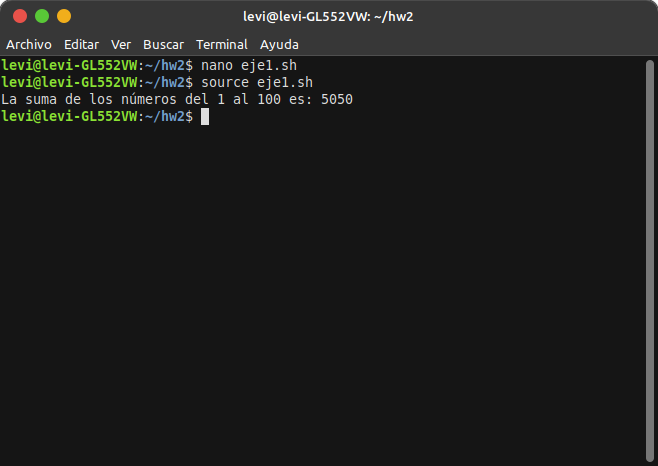
\includegraphics[width=0.8\linewidth]{Tarea2/teje1.png}
    \caption{ compilación del ejercicio 1}
\end{figure}

\newpage
\subsection{Ejercicio 2}
\begin{lstlisting}
#!/bin/bash
# Program Ejercicio 2
# Authors: Gustavo Aguas y Sebastian Paucar
# Explicacion del programa: Este programa cuenta del 1 al 10 utilizando un ciclo while.

count=1

while [ $count -le 10 ]
do
  echo "Número: $count"
  count=$((count + 1))
done
# I love Linux
\end{lstlisting}
\begin{figure}[h]
    \centering
    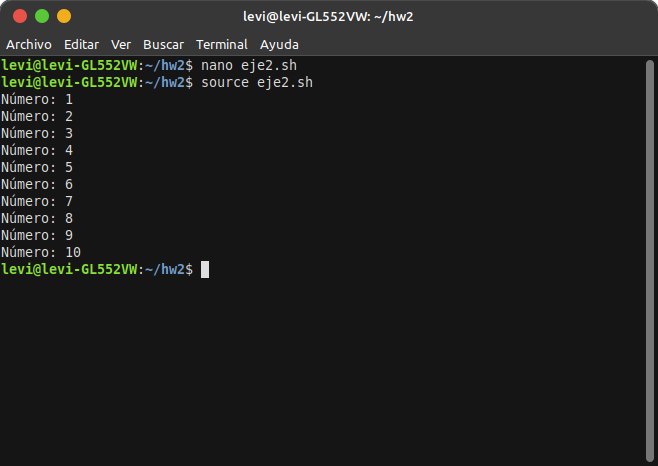
\includegraphics[width=0.8\linewidth]{Tarea2/teje2.png}
    \caption{ compilación del ejercicio 2}
\end{figure}
\newpage
\subsection{Ejercicio 3}
\begin{lstlisting}
#!/bin/bash
# Program Ejercicio 3
# Authors: Gustavo Aguas y Sebastian Paucar
# Explicacion del programa: Este programa verifica si un número ingresado es par o impar.

read -p "Ingresa un número: " num

if [ $((num % 2)) -eq 0 ]; then
  echo "El número $num es par."
else
  echo "El número $num es impar."
fi
#I love linux
\end{lstlisting}
\begin{figure}[h]
    \centering
    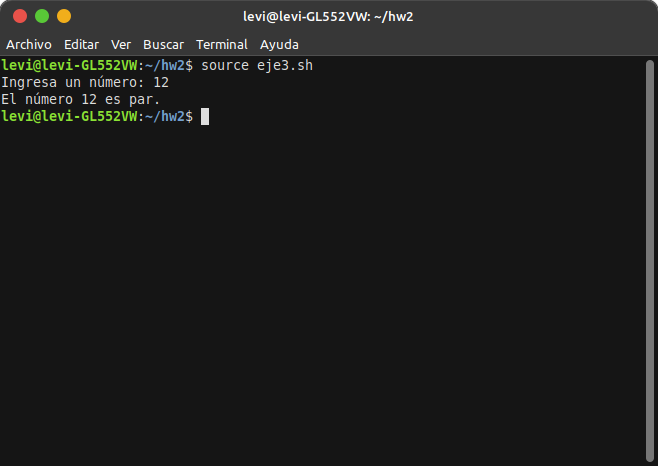
\includegraphics[width=0.8\linewidth]{Tarea2/teje32.png}
    \caption{ compilación del ejercicio 3}
\end{figure}
\newpage
\subsection{Ejercicio 4}
\begin{lstlisting}
#!/bin/bash
# Program Ejercicio 4
# Authors: Gustavo Aguas y Sebastian Paucar
# Explicacion del programa: Este programa muestra los nombres de los días de la semana utilizando un arreglo.

dias=("Lunes" "Martes" "Miércoles" "Jueves" "Viernes" "Sábado" "Domingo")

for dia in "${dias[@]}"
do
  echo "Día: $dia"
done
#I love linux
\end{lstlisting}
\begin{figure}[h]
    \centering
    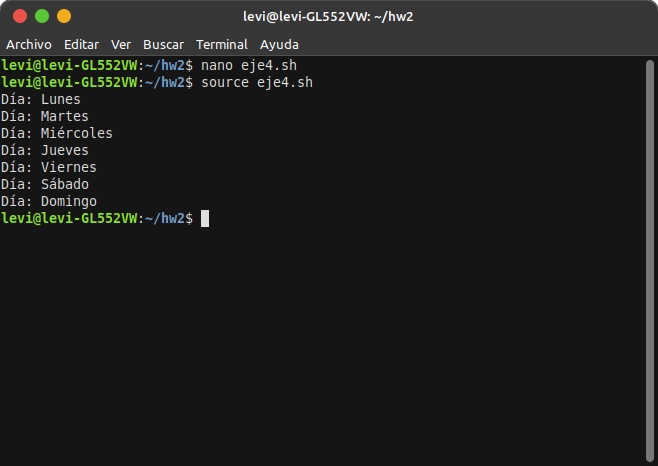
\includegraphics[width=0.8\linewidth]{Tarea2/teje4.png}
    \caption{ compilación del ejercicio 4}
\end{figure}
\newpage
\subsection{Ejercicio 5}
\begin{lstlisting}
#!/bin/bash
# Program Ejercicio 5
# Authors: Gustavo Aguas y Sebastian Paucar
# Explicacion del programa: Este programa imprime la tabla de multiplicar del número ingresado.

read -p "Ingresa un número: " num

for i in {1..10}
do
  echo "$num x $i = $((num * i))"
done
#I love linux
\end{lstlisting}
\begin{figure}[h]
    \centering
    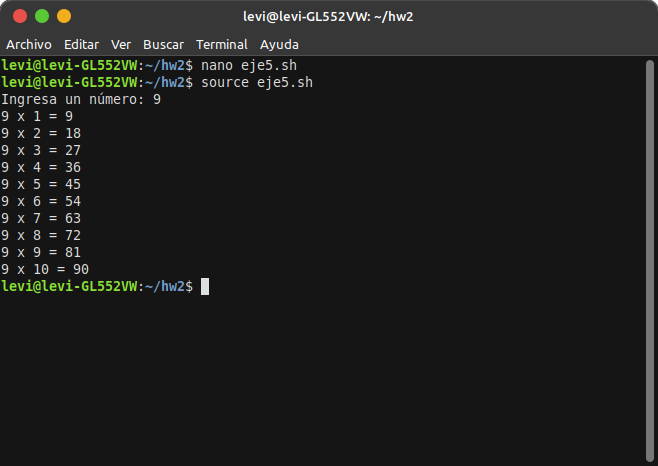
\includegraphics[width=0.8\linewidth]{Tarea2/teje5.png}
    \caption{ compilación del ejercicio 5}
\end{figure}
\newpage
\subsection{Ejercicio 6}

\begin{lstlisting}
#!/bin/bash
# Program Ejercicio 6
# Authors: Gustavo Aguas y Sebastian Paucar
# Explicacion del programa: Este programa encuentra el número más grande en un arreglo.

numeros=(23 45 67 89 12 34 56)

max=${numeros[0]}

for num in "${numeros[@]}"
do
  if [ $num -gt $max ]; then
    max=$num
  fi
done

echo "El número más grande es: $max"
#I love linux
\end{lstlisting}
\begin{figure}[h]
    \centering
    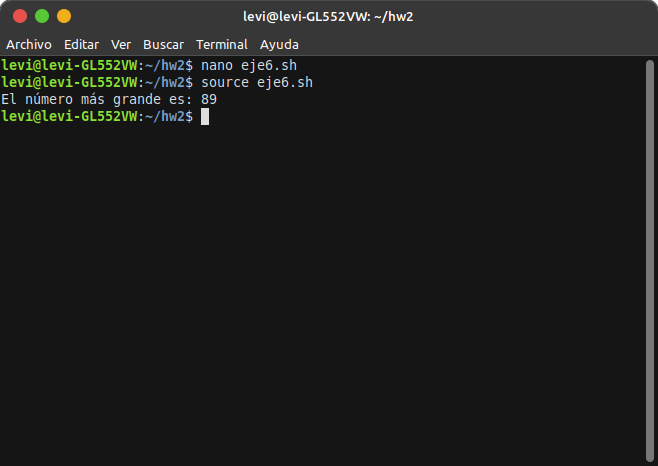
\includegraphics[width=0.8\linewidth]{Tarea2/teje6.png}
    \caption{ compilación del ejercicio 6}
\end{figure}
\newpage
\subsection{Ejercicio 7}
\begin{lstlisting}
#!/bin/bash
# Program Ejercicio 7
# Authors: Gustavo Aguas y Sebastian Paucar
# Explicacion del programa: Este programa cuenta el número de vocales en una cadena ingresada.

read -p "Ingresa una cadena: " cadena

vocales=0

for (( i=0; i<${#cadena}; i++ ))
do
  char=${cadena:$i:1}
  if [[ "$char" =~ [aeiouAEIOU] ]]; then
    vocales=$((vocales + 1))
  fi
done

echo "La cadena contiene $vocales vocales."
#I love linux
\end{lstlisting}
\begin{figure}[h]
    \centering
    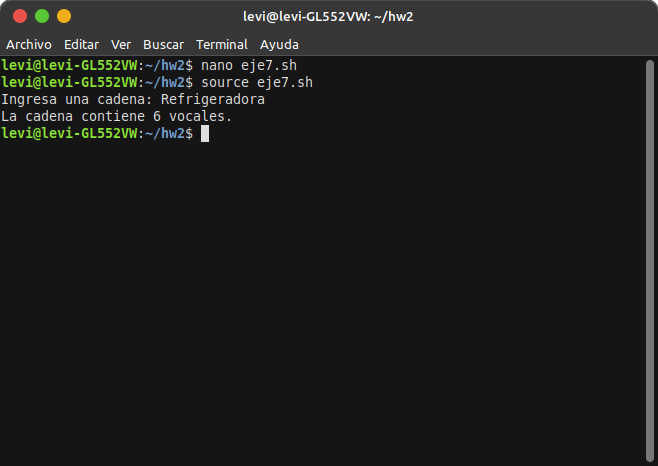
\includegraphics[width=0.8\linewidth]{Tarea2/teje7.png}
    \caption{ compilación del ejercicio 7}
\end{figure}
\newpage
\subsection{Ejercicio 8}
\begin{lstlisting}
#!/bin/bash
# Program Ejercicio 8
# Authors: Gustavo Aguas y Sebastian Paucar
# Explicacion del programa: Este programa verifica si un número ingresado es primo.

read -p "Ingresa un número: " num
es_primo=1

if [ $num -le 1 ]; then
  es_primo=0
else
  for ((i=2; i<=num/2; i++))
  do
    if [ $((num % i)) -eq 0 ]; then
      es_primo=0
      break
    fi
  done
fi

if [ $es_primo -eq 1 ]; then
  echo "El número $num es primo."
else
  echo "El número $num no es primo."
fi
#I love linux
\end{lstlisting}
\begin{figure}[h]
    \centering
    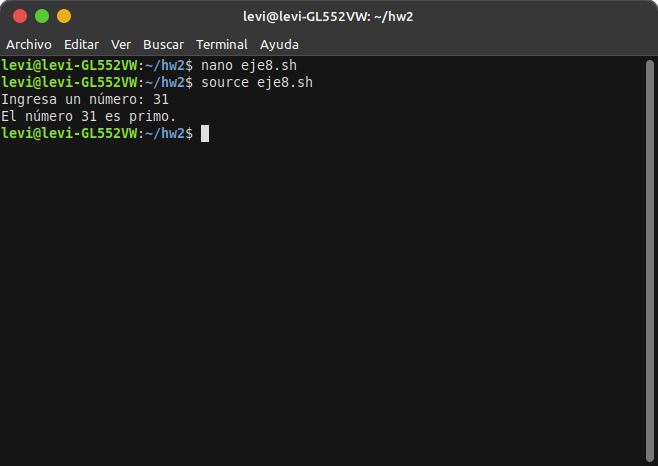
\includegraphics[width=0.6\linewidth]{Tarea2/teje8.png}
    \caption{ compilación del ejercicio 8}
\end{figure}
\newpage
\subsection{Ejercicio 9}
\begin{lstlisting}
#!/bin/bash
# Program Ejercicio 9
# Authors: Gustavo Aguas y Sebastian Paucar
# Explicacion del programa: Este programa invierte una cadena ingresada.

read -p "Ingresa una cadena: " cadena

longitud=${#cadena}

for (( i=$longitud-1; i>=0; i-- ))
do
  invertida="$invertida${cadena:$i:1}"
done

echo "La cadena invertida es: $invertida"
#I love linux
\end{lstlisting}
\begin{figure}[h]
    \centering
    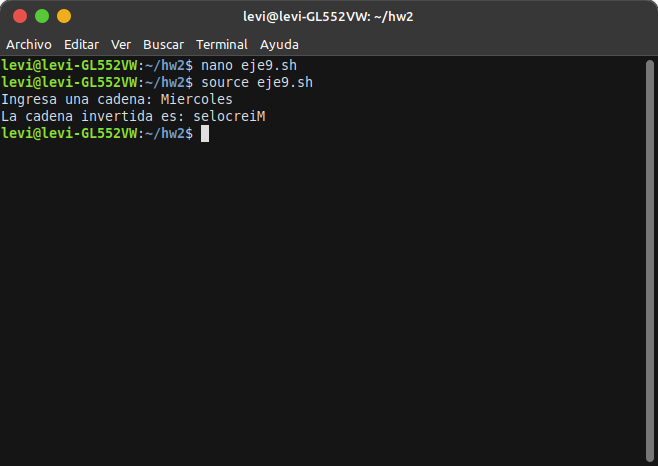
\includegraphics[width=0.8\linewidth]{Tarea2/teje9.png}
    \caption{ compilación del ejercicio 9}
\end{figure}
\newpage
\subsection{Ejercicio 10}

\begin{lstlisting}
#!/bin/bash
# Program Ejercicio 10
# Authors: Gustavo Aguas y Sebastian Paucar
# Explicacion del programa: Este programa calcula el factorial de un número ingresado.

read -p "Ingresa un número: " num
factorial=1

for (( i=1; i<=num; i++ ))
do
  factorial=$((factorial * i))
done

echo "El factorial de $num es: $factorial"
\end{lstlisting}
\begin{figure}[h]
    \centering
    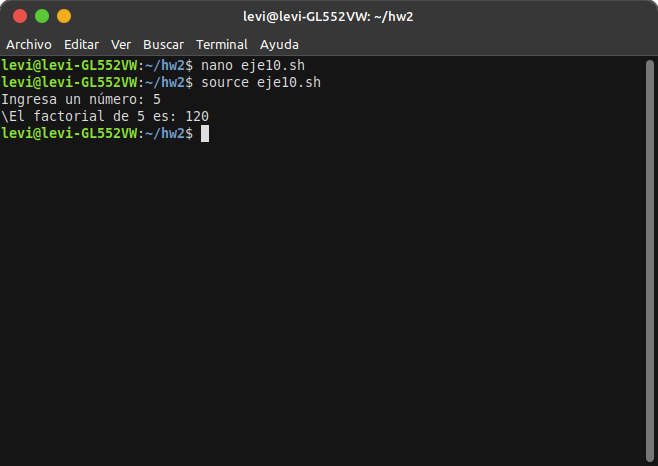
\includegraphics[width=0.8\linewidth]{Tarea2/teje10.png}
    \caption{ compilación del ejercicio 10}
\end{figure}

\newpage
\section{Tarea 2}

\subsection{Ejercicios de programación en Shell con while, if}

Realizar 15 ejercicios

\subsection{Ejercicio 1}

El menor de dos numeros
\begin{lstlisting}
#!/bin/bash
#Program Ejercicio 1
#Authors: Gustavo Aguas y Sebastian Paucar
#Date: 29-05-2023
clear
echo "Ingrese el 1er numero";
read num1;
echo "Ingrese el 2do numero";
read num2;
if [ $num1 -lt $num2 ]; then
echo "el menor  numero es: $num1"
elif [ $num2 -lt $num1 ]; then
echo "El menor es: $num2";
else 
echo "$num1, $num2 son iguales";
fi
#I love linux

\end{lstlisting}
\begin{figure}[h]
    \centering
    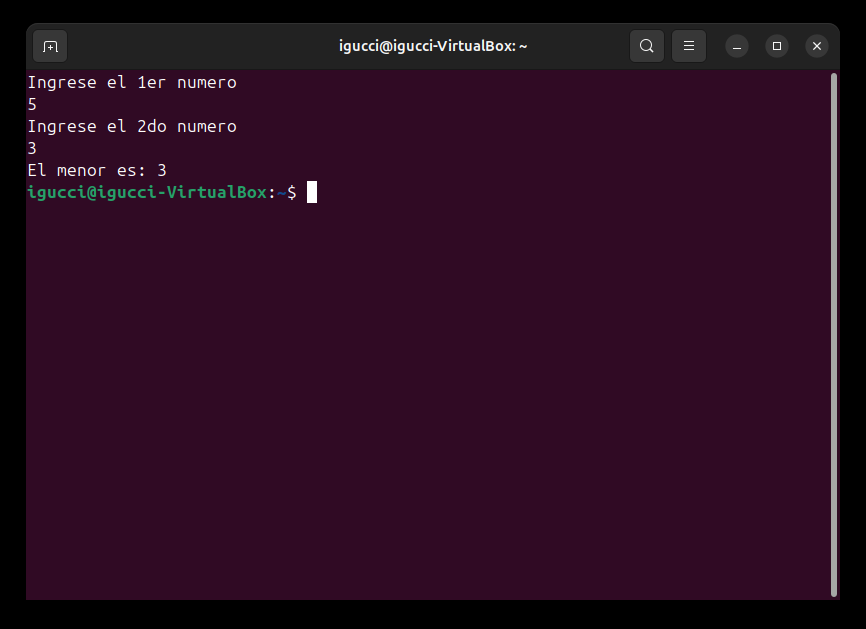
\includegraphics[width=0.5\linewidth]{Ej1.png}
    \caption{Ejercicio 1}
 
\end{figure}


\newpage
\subsection{Ejercicio 2}

Operaciones basicas
\begin{lstlisting}
#!/bin/bash
#Program Ejercicio 2
#Authors: Gustavo Aguas y Sebastian Paucar
#Date: 29-05-2023
echo "Ingrese el primer número entero positivo:"
read num1

echo "Ingrese el segundo número entero positivo:"
read num2

suma=$(expr $num1 + $num2)
resta=$(expr $num1 - $num2)
multiplicacion=$(expr $num1 \* $num2)
division=$(expr $num1 / $num2)

echo "Resultados:"
echo "Suma: $num1 + $num2 = $suma"
echo "Resta: $num1 - $num2 = $resta"
echo "Multiplicación: $num1 * $num2 = $multiplicacion"
echo "División: $num1 / $num2 = $division"

\end{lstlisting}
\begin{figure}[h]
    \centering
    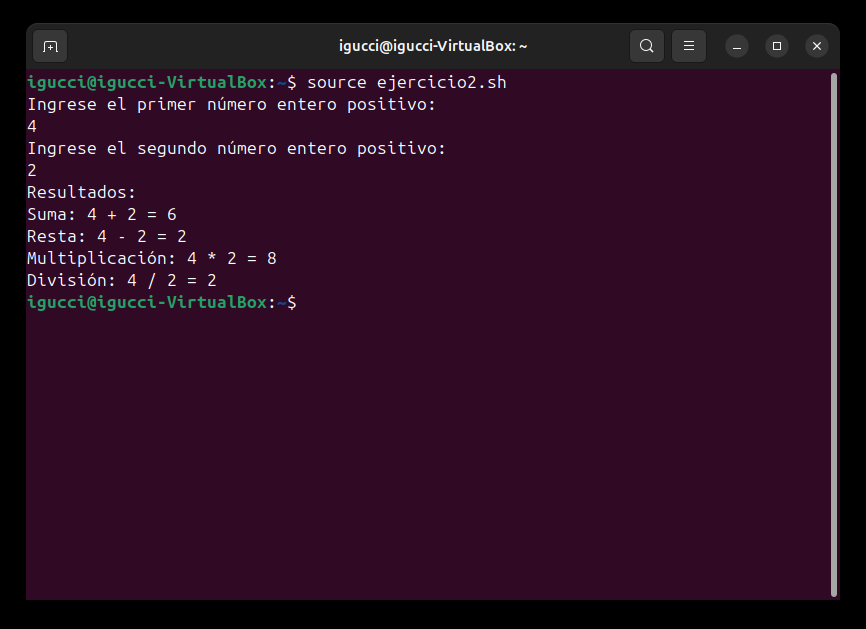
\includegraphics[width=0.5\linewidth]{Ej2.png}
    \caption{Ejercicio 2}

\end{figure}

\newpage
\subsection{Ejercicio 3}

Secuencia hasta el 10
\begin{lstlisting}
#!/bin/bash
#Program Ejercicio 3
#Authors: Gustavo Aguas y Sebastian Paucar
#Date: 29-05-2023
cont=0
while [ $cont -lt 11 ]
do
echo $cont
cont=$((cont + 1))
done
# I LOVE LINUX
\end{lstlisting}
\begin{figure}[h]
    \centering
    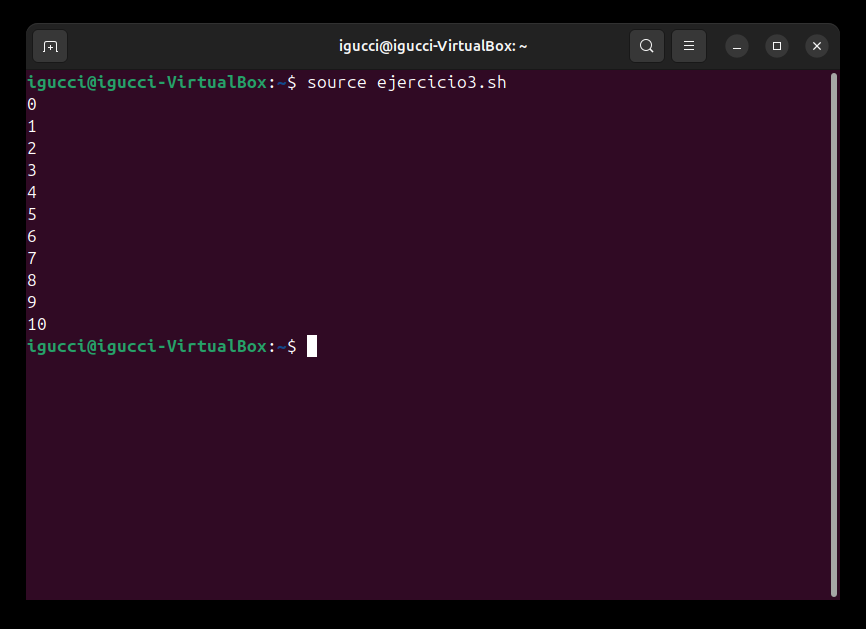
\includegraphics[width=0.5\linewidth]{Ej3.png}
    \caption{Ejercicio 3}

\end{figure}

\newpage
\subsection{Ejercicio 4}

Primeros 20 multiplos de 3
\begin{lstlisting}
#!/bin/bash
#Program Ejercicio 4
#Authors: Gustavo Aguas y Sebastian Paucar
#Date: 29-05-2023
# Imprimir los primeros 20 múltiplos de 3
echo "Los primeros 20 múltiplos de 3 son:"
for (( i=1; i<=20; i++ )); do
  multiplo=$((i * 3))
  echo $multiplo
done

\end{lstlisting}
\begin{figure}[h]
    \centering
    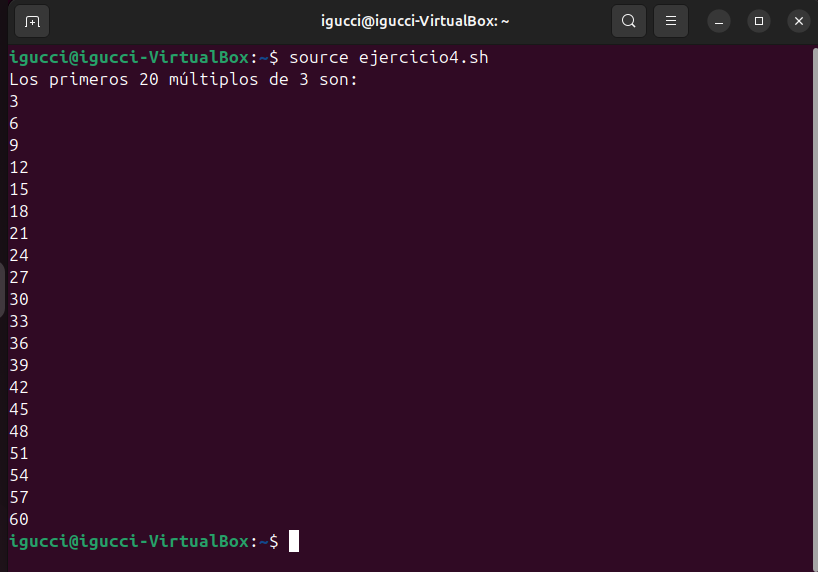
\includegraphics[width=0.5\linewidth]{Ej4.png}
    \caption{Ejercicio 4}

\end{figure}

\newpage
\subsection{Ejercicio 5}

Tabla de multiplicar del num 4 hasta el  20
\begin{lstlisting}
#!/bin/bash
#Program Ejercicio 5
#Authors: Gustavo Aguas y Sebastian Paucar
#Date: 29-05-2023
# Leer un número entero positivo
echo "Ingrese un número entero positivo:"
read num

# Calcular y mostrar la tabla de multiplicar hasta el 20
for ((i = 1; i <= 20; i++)); do
  resultado=$((num * i))
  echo "$num x $i = $resultado"
done

\end{lstlisting}
\begin{figure}[h]
    \centering
    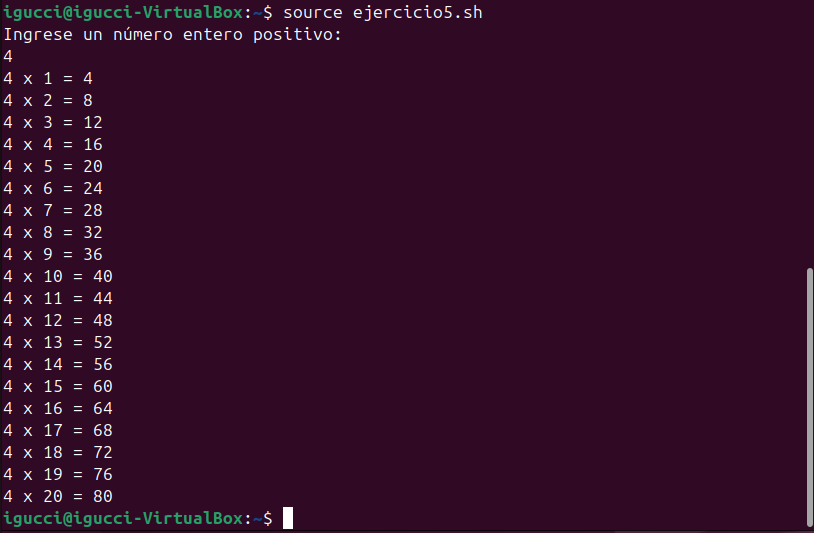
\includegraphics[width=0.5\linewidth]{Ej5.png}
    \caption{Ejercicio 5}

\end{figure}
\newpage
\subsection{Ejercicio 6}
Verificar si un número es positivo, negativo o cero

\begin{lstlisting}
#!/bin/bash
#Program Ejercicio 6
#Authors: Gustavo Aguas y Sebastian Paucar
#Date: 29-05-2023
echo "Ingrese un número:"
read num

if (( num > 0 )); then
  echo "$num es positivo"
elif (( num < 0 )); then
  echo "$num es negativo"
else
  echo "$num es cero"
fi

echo "I love Linux"


\end{lstlisting}
\begin{figure}[h]
    \centering
    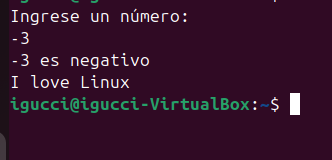
\includegraphics[width=0.5\linewidth]{image.png}
    \caption{Ejercicio 6}
\end{figure}
\newpage
\subsection{Ejercicio 7}

Imprimir los primeros 10 números pares y su suma 
\begin{lstlisting}
#!/bin/bash
#Program Ejercicio 7
#Authors: Gustavo Aguas y Sebastian Paucar
#Date: 29-05-2023
suma=0
for (( i = 1; i <= 10; i++ )); do
  num=$(( i * 2 ))
  echo "Número par: $num"
  suma=$(( suma + num ))
done

echo "La suma de los primeros 10 números pares es $suma"

echo "I love Linux"

\end{lstlisting}
\begin{figure}[h]
    \centering
    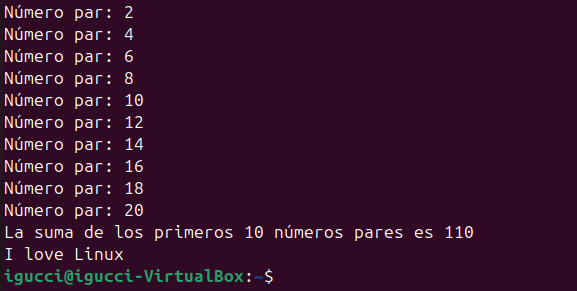
\includegraphics[width=0.5\linewidth]{Ej7.png}
    \caption{Ejercicio 7}
\end{figure}
\newpage
\subsection{Ejercicio 8}

Contar del 1 al 20 y mostrar si cada número es par o impar
\begin{lstlisting}
#!/bin/bash
#Program Ejercicio 8
#Authors: Gustavo Aguas y Sebastian Paucar
#Date: 29-05-2023
for (( i = 1; i <= 20; i++ )); do
  if (( i % 2 == 0 )); then
    echo "$i es par"
  else
    echo "$i es impar"
  fi
done

echo "I love Linux"

\end{lstlisting}
\begin{figure}[h]
    \centering
    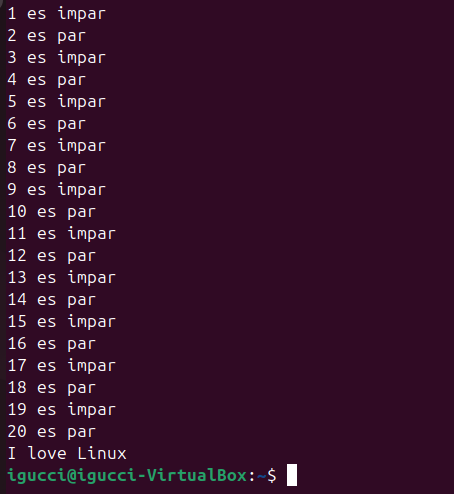
\includegraphics[width=0.5\linewidth]{Ej8.png}
    \caption{Ejercicio 8}
\end{figure}
\newpage
\subsection{Ejercicio 9}
 Calcular la suma de los números del 1 al 100 y mostrar el resultado
\begin{lstlisting}
#!/bin/bash
#Program Ejercicio 9
#Authors: Gustavo Aguas y Sebastian Paucar
#Date: 29-05-2023
suma=0
for (( i = 1; i <= 100; i++ )); do
  suma=$(( suma + i ))
done

echo "La suma de los números del 1 al 100 es $suma"

echo "I love Linux"

\end{lstlisting}

\begin{figure}[h]
    \centering
    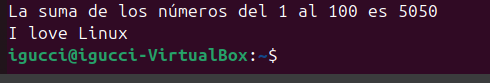
\includegraphics[width=0.5\linewidth]{Ej9.png}
    \caption{Ejercicio 9}
\end{figure}
\newpage
\subsection{Ejercicio 10}
Imprimir la tabla de multiplicar de un número hasta el 20

\begin{lstlisting}
#!/bin/bash
#Program Ejercicio 10
#Authors: Gustavo Aguas y Sebastian Paucar
#Date: 29-05-2023
echo "Ingrese un número entero positivo:"
read num

for (( i = 1; i <= 20; i++ )); do
  resultado=$(( num * i ))
  echo "$num x $i = $resultado"
done

echo "I love Linux"

\end{lstlisting}

\begin{figure}[h]
    \centering
    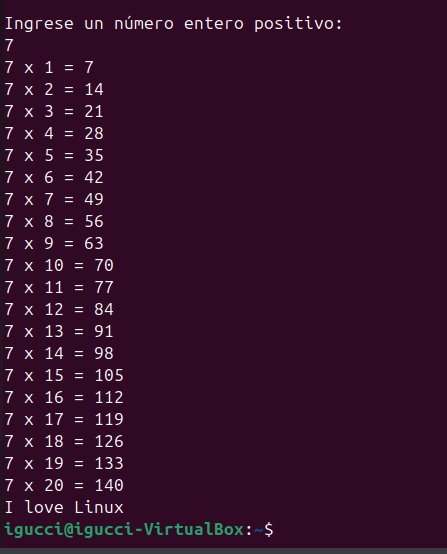
\includegraphics[width=0.5\linewidth]{Ej10.png}
    \caption{Ejercicio 10}
\end{figure}
\newpage
\subsection{Ejercicio 11}
Contar las letras de una cadena y mostrar cuántas son vocales y cuántas son consonantes

\begin{lstlisting}
#!/bin/bash
#Program Ejercicio 11
#Authors: Gustavo Aguas y Sebastian Paucar
#Date: 29-05-2023
echo "Ingrese una cadena de texto:"
read cadena

longitud=${#cadena}
vocales=0
consonantes=0

for (( i = 0; i < longitud; i++ )); do
  letra=${cadena:$i:1}
  if [[ $letra =~ [aeiouAEIOU] ]]; then
    vocales=$(( vocales + 1 ))
  elif [[ $letra =~ [bcdfghjklmnpqrstvwxyzBCDFGHJKLMNPQRSTVWXYZ] ]]; then
    consonantes=$(( consonantes + 1 ))
  fi
done

echo "La cadena tiene $longitud caracteres, de los cuales $vocales son vocales y $consonantes son consonantes."

echo "I love Linux"


\end{lstlisting}
\begin{figure}[h]
    \centering
    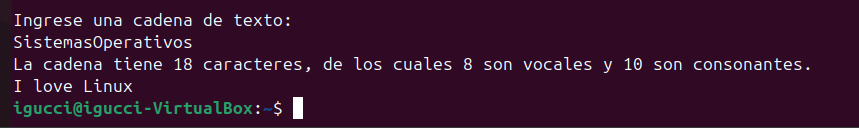
\includegraphics[width=1\linewidth]{Ej11.png}
    \caption{Ejercicio 11}
\end{figure}
\newpage
\subsection{Ejercicio 12}

Comprobar si un número es múltiplo de 3 o 5 y mostrar todos los múltiplos de 3 o 5 hasta 50

\begin{lstlisting}
#!/bin/bash
#Program Ejercicio 12
#Authors: Gustavo Aguas y Sebastian Paucar
#Date: 29-05-2023
echo "Ingrese un número:"
read num

if (( num % 3 == 0 )); then
  echo "$num es múltiplo de 3"
elif (( num % 5 == 0 )); then
  echo "$num es múltiplo de 5"
else
  echo "$num no es múltiplo de 3 ni de 5"
fi

echo "Múltiplos de 3 o 5 hasta 50:"
for (( i = 1; i <= 50; i++ )); do
  if (( i % 3 == 0 || i % 5 == 0 )); then
    echo $i
  fi
done

echo "I love Linux"

\end{lstlisting}
\begin{figure}[h]
    \centering
    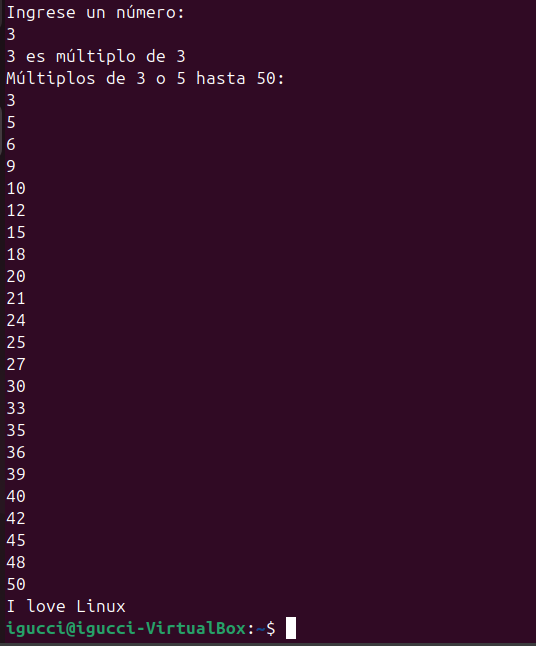
\includegraphics[width=0.5\linewidth]{Ej12.png}
    \caption{Ejercicio 12}
\end{figure}
\newpage
\subsection{Ejercicio 13}
Sumar los primeros N números pares
\begin{lstlisting}
#!/bin/bash
#Program Ejercicio 13
#Authors: Gustavo Aguas y Sebastian Paucar
#Date: 29-05-2023
echo "Ingrese un número entero positivo N:"
read N

suma=0
for (( i = 1; i <= N; i++ )); do
  num=$(( i * 2 ))
  suma=$(( suma + num ))
done

echo "La suma de los primeros $N números pares es $suma"

echo "I love Linux"

\end{lstlisting}
\begin{figure}[h]
    \centering
    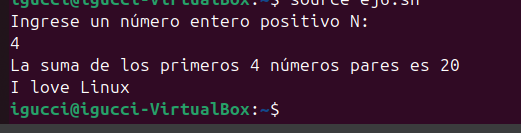
\includegraphics[width=1\linewidth]{Ej13.png}
    \caption{Ejercicio 13}
\end{figure}
\newpage
\subsection{Ejercicio 14}
Imprimir los números primos del 1 al 50
\begin{lstlisting}
#!/bin/bash
#Program Ejercicio 14
#Authors: Gustavo Aguas y Sebastian Paucar
#Date: 29-05-2023
echo "Números primos del 1 al 50:"
for (( num = 2; num <= 50; num++ )); do
  es_primo=1
  for (( i = 2; i <= num / 2; i++ )); do
    if (( num % i == 0 )); then
      es_primo=0
      break
    fi
  done
  if (( es_primo == 1 )); then
    echo $num
  fi
done

echo "I love Linux"

\end{lstlisting}
\begin{figure}[h]
    \centering
    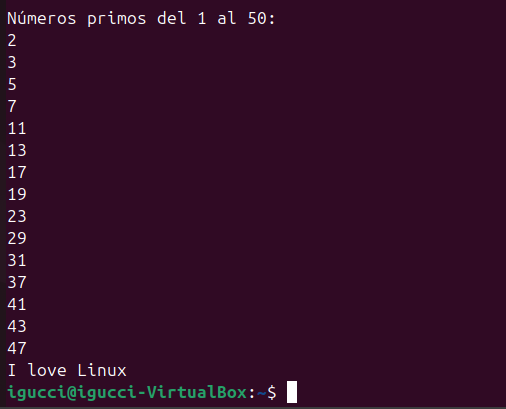
\includegraphics[width=0.5\linewidth]{Ej14.png}
    \caption{Ejercicio 14}
\end{figure}
\newpage
\subsection{Ejercicio 15}
Verificar si una cadena es un palíndromo
\begin{lstlisting}
#!/bin/bash
#Program Ejercicio 15
#Authors: Gustavo Aguas y Sebastian Paucar
#Date: 29-05-2023
echo "Ingrese una cadena de texto:"
read cadena

cadena_invertida=$(echo $cadena | rev)

if [ "$cadena" == "$cadena_invertida" ]; then
  echo "La cadena es un palíndromo"
else
  echo "La cadena no es un palíndromo"
fi

echo "I love Linux"

\end{lstlisting}
\begin{figure}[h]
    \centering
    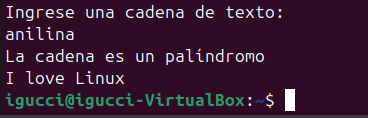
\includegraphics[width=0.5\linewidth]{Ej15.png}
    \caption{Ejercicio 15}
\end{figure}
\newpage
\section{Tarea 3}
\subsection{Ejercicios de series}
Realizar 10 ejercicios
\subsection{Ejercicio 1}
\begin{lstlisting}
#!/bin/bash
# Program Ejercicio 1
# Authors: Gustavo Aguas y Sebastian Paucar
# Explicacion del programa: Serie de números del 1 al 20 y su suma total
sum=0
for i in {1..20}; do
    echo $i
    sum=$((sum + i))
done
echo "La suma total es: $sum"
# I love Linux
\end{lstlisting}
\begin{figure}[h]
    \centering
    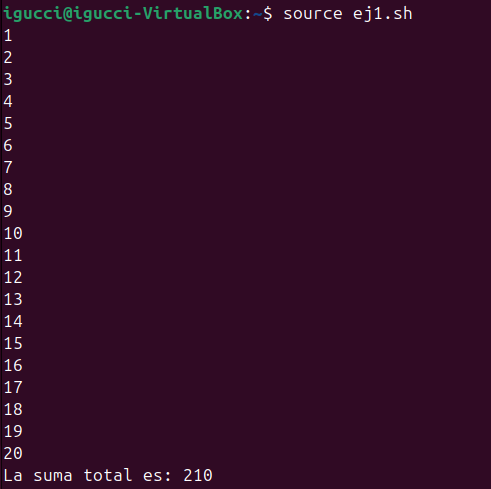
\includegraphics[width=0.6\linewidth]{series/ej1.png}
    \caption{Ejercicio 1}
\end{figure}

\newpage
\subsection{Ejercicio 2}
\begin{lstlisting}
#!/bin/bash
# Program Ejercicio 2
# Authors: Gustavo Aguas y Sebastian Paucar
# Explicacion del programa: Serie de números pares del 2 al 40 y su promedio
sum=0
count=0
for i in {2..40..2}; do
    echo $i
    sum=$((sum + i))
    count=$((count + 1))
done
average=$(echo "scale=2; $sum / $count" | bc)
echo "El promedio es: $average"
# I love Linux
\end{lstlisting}
\begin{figure}[h]
    \centering
    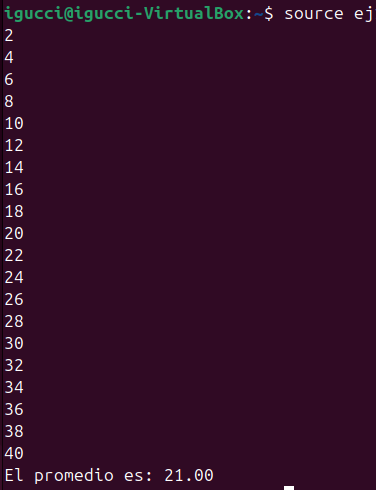
\includegraphics[width=0.5\linewidth]{series/ej2.png}
    \caption{Ejercicio 2}
\end{figure}
\newpage
\subsection{Ejercicio 3}
\begin{lstlisting}
#!/bin/bash
# Program Ejercicio 3
# Authors: Gustavo Aguas y Sebastian Paucar
# Explicacion del programa: Serie de números impares del 1 al 39 y su producto total

product=1
for i in {1..39..2}; do
    echo $i
    product=$((product * i))
done
echo "El producto total es: $product"
#I love linux
\end{lstlisting}
\begin{figure}[h]
    \centering
    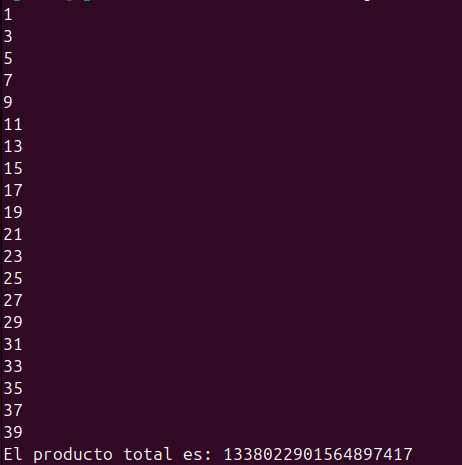
\includegraphics[width=0.75\linewidth]{series/ej3.png}
    \caption{Ejercicio 3}
\end{figure}
\newpage
\subsection{Ejercicio 4}
\begin{lstlisting}
#!/bin/bash
# Program Ejercicio 4
# Authors: Gustavo Aguas y Sebastian Paucar
# Explicacion del programa: Serie de múltiplos de 3 hasta 60 y contar cuántos hay

count=0
for ((i=3; i<=60; i+=3)); do
    echo $i
    count=$((count + 1))
done
echo "El número de múltiplos de 3 es: $count"
#I love linux
\end{lstlisting}
\begin{figure}[h]
    \centering
    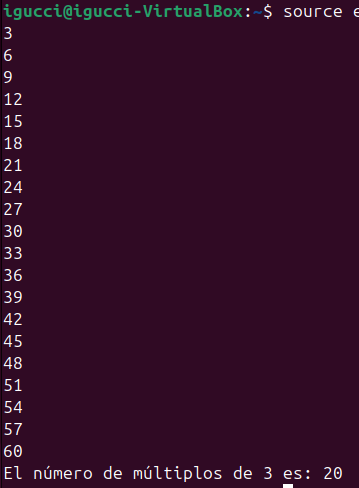
\includegraphics[width=0.5\linewidth]{series/ej4.png}
    \caption{Ejercicio 4}
\end{figure}
\newpage
\subsection{Ejercicio 5}
\begin{lstlisting}
#!/bin/bash
# Program Ejercicio 5
# Authors: Gustavo Aguas y Sebastian Paucar
# Explicacion del programa: Serie de Fibonacci (los primeros 15 números) y su suma

a=0
b=1
sum=$a
echo $a
echo $b
for ((i=2; i<15; i++)); do
    c=$((a + b))
    echo $c
    sum=$((sum + c))
    a=$b
    b=$c
done
echo "La suma de la serie Fibonacci es: $sum"
#I love linux
\end{lstlisting}
\begin{figure}[h]
    \centering
    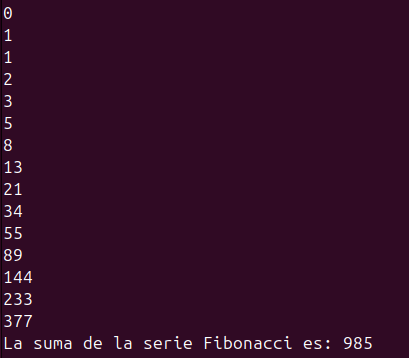
\includegraphics[width=0.75\linewidth]{series/ej5.png}
    \caption{Ejercicio 5}
\end{figure}
\newpage
\subsection{Ejercicio 6}

\begin{lstlisting}
#!/bin/bash
# Program Ejercicio 6
# Authors: Gustavo Aguas y Sebastian Paucar
# Explicacion del programa: Serie de cuadrados de los números del 1 al 15 y su suma

sum=0
for i in {1..15}; do
    square=$(echo "$i^2" | bc)
    echo "$i^2 = $square"
    sum=$(echo "$sum + $square" | bc)
done
echo "La suma de los cuadrados es: $sum"
#I love linux
\end{lstlisting}
\begin{figure}[h]
    \centering
    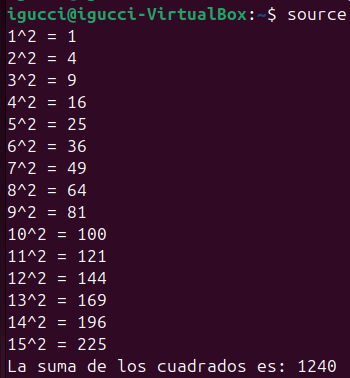
\includegraphics[width=0.75\linewidth]{series/ej6.png}
    \caption{Ejercicio 6}
\end{figure}
\newpage
\subsection{Ejercicio 7}
\begin{lstlisting}
#!/bin/bash
# Program Ejercicio 7
# Authors: Gustavo Aguas y Sebastian Paucar
# Explicacion del programa: Serie de cubos de los números del 1 al 10 y su promedio

sum=0
count=0
for i in {1..10}; do
    cube=$(echo "$i^3" | bc)
    echo "$i^3 = $cube"
    sum=$(echo "$sum + $cube" | bc)
    count=$((count + 1))
done
average=$(echo "scale=2; $sum / $count" | bc)
echo "El promedio de los cubos es: $average"
#I love linux
\end{lstlisting}
\begin{figure}[h]
    \centering
    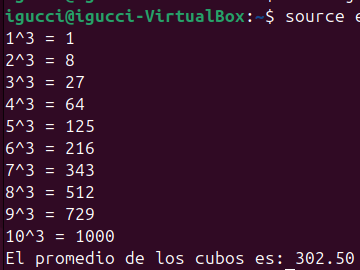
\includegraphics[width=0.6\linewidth]{series/ej7.png}
    \caption{Ejercicio 7}
\end{figure}
\newpage
\subsection{Ejercicio 8}
\begin{lstlisting}
#!/bin/bash
# Program Ejercicio 8
# Authors: Gustavo Aguas y Sebastian Paucar
# Explicacion del programa: Serie de los primeros 10 números con dos decimales y su suma

sum=0
for i in {1..10}; do
    value=$(echo "scale=2; $i/1" | bc)
    echo $value
    sum=$(echo "$sum + $value" | bc)
done
echo "La suma total es: $sum"
#I love linux
\end{lstlisting}
\begin{figure}[h]
    \centering
    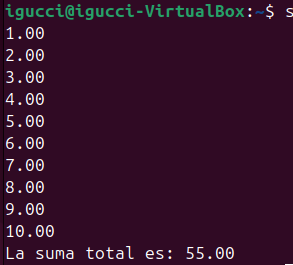
\includegraphics[width=0.6\linewidth]{series/ej8.png}
    \caption{Ejercicio 8}
\end{figure}
\newpage
\subsection{Ejercicio 9}
\begin{lstlisting}
#!/bin/bash
# Program Ejercicio 9
# Authors: Gustavo Aguas y Sebastian Paucar
# Explicacion del programa: Serie de los primeros 10 números factoriales y su suma

factorial() {
    if [ $1 -le 1 ]; then
        echo 1
    else
        echo "$1 * $(factorial $(($1 - 1)))" | bc
    fi
}

sum=0
for i in {1..10}; do
    fact=$(factorial $i)
    echo "$i! = $fact"
    sum=$(echo "$sum + $fact" | bc)
done
echo "La suma de los factoriales es: $sum"
#I love linux
\end{lstlisting}
\begin{figure}[h]
    \centering
    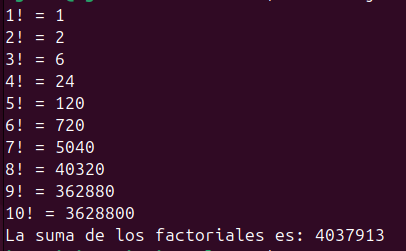
\includegraphics[width=0.6\linewidth]{series/ej9.png}
    \caption{Ejercicio 9}
\end{figure}
\newpage
\subsection{Ejercicio 10}

\begin{lstlisting}
#!/bin/bash
# Program Ejercicio 10
# Authors: Gustavo Aguas y Sebastian Paucar
# Explicacion del programa: Serie de los primeros 10 números con raíz cuadrada y su suma

sum=0
for i in {1..10}; do
    sqrt=$(echo "scale=2; sqrt($i)" | bc)
    echo "sqrt($i) = $sqrt"
    sum=$(echo "$sum + $sqrt" | bc)
done
echo "La suma de las raíces cuadradas es: $sum"
#I love linux
\end{lstlisting}
\begin{figure}[h]
    \centering
    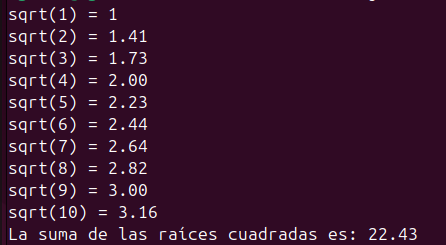
\includegraphics[width=0.75\linewidth]{series/ej10.png}
    \caption{Ejercicio 10}
\end{figure}

\newpage
\section{Tarea 4}
\subsection{Permisos numericos}
Realizar 10 ejercicios
\subsection{Ejercicio 1}
\begin{lstlisting}
#!/bin/bash
# Program Ejercicio 1
# Authors: Gustavo Aguas y Sebastian Paucar
# Explicacion del programa: Crear un archivo file1.txt y otorgarle permisos de lectura, escritura y ejecución al usuario; solo lectura y ejecución al grupo y sin permisos a otros:

touch file1.txt
chmod 750 file1.txt
ls -l file1.txt
# I love Linux
\end{lstlisting}
\begin{figure}[h]
    \centering
    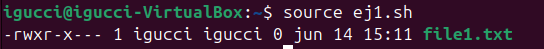
\includegraphics[width=1\linewidth]{pnum/ej1.png}
    \caption{Ejercicio 1}
\end{figure}


\subsection{Ejercicio 2}
\begin{lstlisting}
#!/bin/bash
# Program Ejercicio 2
# Authors: Gustavo Aguas y Sebastian Paucar
# Explicacion del programa: Crear un archivo file2.txt y otorgarle permisos de lectura y escritura al usuario; solo lectura al grupo y sin permisos a otros:

touch file2.txt
chmod 640 file2.txt
ls -l file2.txt
# I love Linux
\end{lstlisting}
\begin{figure}[h]
    \centering
    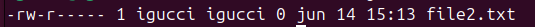
\includegraphics[width=1\linewidth]{pnum/ej2.png}
    \caption{Ejercicio 2}
\end{figure}

\subsection{Ejercicio 3}
\begin{lstlisting}
#!/bin/bash
# Program Ejercicio 3
# Authors: Gustavo Aguas y Sebastian Paucar
# Explicacion del programa: Crear un archivo file3.txt y otorgarle permisos de lectura y escritura al usuario; sin permisos al grupo y otros:

touch file3.txt
chmod 600 file3.txt
ls -l file3.txt
#I love linux
\end{lstlisting}
\begin{figure}[h]
    \centering
    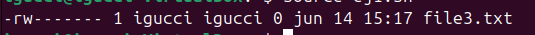
\includegraphics[width=1\linewidth]{pnum/ej3.png}
    \caption{Ejercicio 3}
\end{figure}

\subsection{Ejercicio 4}
\begin{lstlisting}
#!/bin/bash
# Program Ejercicio 4
# Authors: Gustavo Aguas y Sebastian Paucar
# Explicacion del programa: Crear un archivo file4.txt y otorgarle permisos de lectura, escritura y ejecución al usuario y grupo; solo lectura y ejecución a otros:

touch file4.txt
chmod 775 file4.txt
ls -l file4.txt
#I love linux
\end{lstlisting}
\begin{figure}[h]
    \centering
    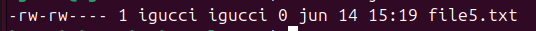
\includegraphics[width=1\linewidth]{pnum/ej5.png}
    \caption{Ejercicio 4}
\end{figure}

\subsection{Ejercicio 5}
\begin{lstlisting}
#!/bin/bash
# Program Ejercicio 5
# Authors: Gustavo Aguas y Sebastian Paucar
# Explicacion del programa: Crear un archivo file5.txt y otorgarle permisos de lectura y escritura al usuario y grupo; sin permisos a otros:

touch file5.txt
chmod 660 file5.txt
ls -l file5.txt
#I love linux
\end{lstlisting}
\begin{figure}[h]
    \centering
    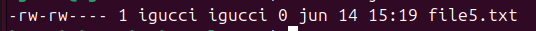
\includegraphics[width=1\linewidth]{pnum/ej5.png}
    \caption{Ejercicio 5}
\end{figure}

\subsection{Ejercicio 6}

\begin{lstlisting}
#!/bin/bash
# Program Ejercicio 6
# Authors: Gustavo Aguas y Sebastian Paucar
# Explicacion del programa: Crear un archivo file6.txt y otorgarle permisos de solo lectura a todos:
bash

touch file6.txt
chmod 444 file6.txt
ls -l file6.txt
#I love linux
\end{lstlisting}
\begin{figure}[h]
    \centering
    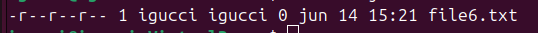
\includegraphics[width=1\linewidth]{pnum/ej6.png}
    \caption{Ejercicio 6}
\end{figure}

\subsection{Ejercicio 7}
\begin{lstlisting}
#!/bin/bash
# Program Ejercicio 7
# Authors: Gustavo Aguas y Sebastian Paucar
# Explicacion del programa: Crear un archivo file7.txt y otorgarle permisos de escritura y ejecución al usuario; solo ejecución al grupo y otros:

touch file7.txt
chmod 311 file7.txt
ls -l file7.txt
#I love linux
\end{lstlisting}
\begin{figure}[h]
    \centering
    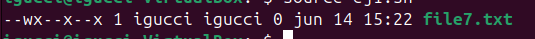
\includegraphics[width=1\linewidth]{pnum/ej7.png}
    \caption{Ejercicio 7}
\end{figure}

\subsection{Ejercicio 8}
\begin{lstlisting}
#!/bin/bash
# Program Ejercicio 8
# Authors: Gustavo Aguas y Sebastian Paucar
# Explicacion del programa: Crear un archivo file8.txt y otorgarle permisos de lectura y ejecución al usuario; solo ejecución al grupo y sin permisos a otros:

touch file8.txt
chmod 510 file8.txt
ls -l file8.txt
#I love linux
\end{lstlisting}
\begin{figure}[h]
    \centering
    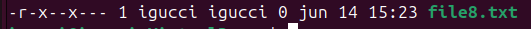
\includegraphics[width=1\linewidth]{pnum/ej8.png}
    \caption{Ejercicio 8}
\end{figure}

\subsection{Ejercicio 9}
\begin{lstlisting}
#!/bin/bash
# Program Ejercicio 9
# Authors: Gustavo Aguas y Sebastian Paucar
# Explicacion del programa: Crear un archivo file9.txt y otorgarle permisos de lectura y escritura al usuario; solo lectura y escritura al grupo y sin permisos a otros:

touch file9.txt
chmod 660 file9.txt
ls -l file9.txt
#I love linux
\end{lstlisting}
\begin{figure}[h]
    \centering
    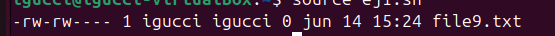
\includegraphics[width=1\linewidth]{pnum/ej9.png}
    \caption{Ejercicio 9}
\end{figure}
\newpage
\subsection{Ejercicio 10}
\begin{lstlisting}
#!/bin/bash
# Program Ejercicio 10
# Authors: Gustavo Aguas y Sebastian Paucar
# Explicacion del programa: Crear un archivo file10.txt y otorgarle permisos de lectura y ejecución al usuario y grupo; sin permisos a otros:

touch file10.txt
chmod 550 file10.txt
ls -l file10.txt
#I love linux
\end{lstlisting}
\begin{figure}[h]
    \centering
    
\includegraphics[width=1\linewidth]{pnum/ej10.png}
    \caption{Ejercicio 10}
\end{figure}
\newpage
\section{Tarea 5}
\subsection{Permisos Simbolicos}
Realizar 10 ejercicios
\subsection{Ejercicio 1}
\begin{lstlisting}
#!/bin/bash
# Program Ejercicio 1
# Authors: Gustavo Aguas y Sebastian Paucar
# Explicacion del programa: Crear un archivo file1.txt y otorgarle permisos de lectura y escritura al usuario; solo lectura al grupo y sin permisos a otros:

touch file1.txt
chmod u=rw,g=r,o= file1.txt
ls -l file1.txt
# I love Linux
\end{lstlisting}
\begin{figure}[h]
    \centering
    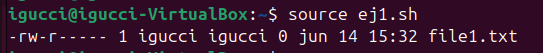
\includegraphics[width=1\linewidth]{psimb/ej1.png}
    \caption{Ejercicio 1}
\end{figure}


\subsection{Ejercicio 2}
\begin{lstlisting}
#!/bin/bash
# Program Ejercicio 2
# Authors: Gustavo Aguas y Sebastian Paucar
# Explicacion del programa: Crear un archivo file2.txt y otorgarle permisos de lectura, escritura y ejecución al usuario y grupo; solo lectura a otros:

touch file2.txt
chmod u=rwx,g=rwx,o=r file2.txt
ls -l file2.txt
# I love Linux
\end{lstlisting}
\begin{figure}[h]
    \centering
    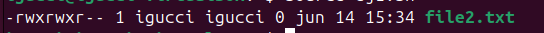
\includegraphics[width=1\linewidth]{psimb/ej2.png}
    \caption{Ejercicio 2}
\end{figure}

\subsection{Ejercicio 3}
\begin{lstlisting}
#!/bin/bash
# Program Ejercicio 3
# Authors: Gustavo Aguas y Sebastian Paucar
# Explicacion del programa: Crear un archivo file3.txt y otorgarle permisos de solo lectura al usuario; sin permisos al grupo y otros:

touch file3.txt
chmod u=r,g=,o= file3.txt
ls -l file3.txt
#I love linux
\end{lstlisting}
\begin{figure}[h]
    \centering
    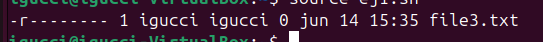
\includegraphics[width=1\linewidth]{psimb/ej3.png}
    \caption{Ejercicio 3}
\end{figure}

\subsection{Ejercicio 4}
\begin{lstlisting}
#!/bin/bash
# Program Ejercicio 4
# Authors: Gustavo Aguas y Sebastian Paucar
# Explicacion del programa: Crear un archivo file4.txt y otorgarle permisos de lectura y ejecución al usuario y grupo; sin permisos a otros:

touch file4.txt
chmod u=rx,g=rx,o= file4.txt
ls -l file4.txt
#I love linux
\end{lstlisting}
\begin{figure}[h]
    \centering
    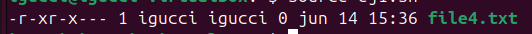
\includegraphics[width=1\linewidth]{psimb/ej4.png}
    \caption{Ejercicio 4}
\end{figure}

\subsection{Ejercicio 5}
\begin{lstlisting}
#!/bin/bash
# Program Ejercicio 5
# Authors: Gustavo Aguas y Sebastian Paucar
# Explicacion del programa: Crear un archivo file5.txt y otorgarle permisos de escritura y ejecución al usuario; solo ejecución al grupo y otros:

touch file5.txt
chmod u=wx,g=x,o=x file5.txt
ls -l file5.txt
#I love linux
\end{lstlisting}
\begin{figure}[h]
    \centering
    \includegraphics[width=1\linewidth]{psimb/ej5.png}
    \caption{Ejercicio 5}
\end{figure}

\subsection{Ejercicio 6}

\begin{lstlisting}
#!/bin/bash
# Program Ejercicio 6
# Authors: Gustavo Aguas y Sebastian Paucar
# Explicacion del programa: Crear un archivo file6.txt y otorgarle permisos de lectura y escritura al usuario y grupo; sin permisos a otros:

touch file6.txt
chmod u=rw,g=rw,o= file6.txt
ls -l file6.txt
#I love linux
\end{lstlisting}
\begin{figure}[h]
    \centering
    \includegraphics[width=1\linewidth]{psimb/ej6.png}
    \caption{Ejercicio 6}
\end{figure}

\subsection{Ejercicio 7}
\begin{lstlisting}
#!/bin/bash
# Program Ejercicio 7
# Authors: Gustavo Aguas y Sebastian Paucar
# Explicacion del programa: Crear un archivo file7.txt y otorgarle permisos de solo lectura a todos:

touch file7.txt
chmod u=r,g=r,o=r file7.txt
ls -l file7.txt
#I love linux
\end{lstlisting}
\begin{figure}[h]
    \centering
    \includegraphics[width=1\linewidth]{psimb/ej7.png}
    \caption{Ejercicio 7}
\end{figure}
\newpage
\subsection{Ejercicio 8}
\begin{lstlisting}
#!/bin/bash
# Program Ejercicio 8
# Authors: Gustavo Aguas y Sebastian Paucar
# Explicacion del programa: Crear un archivo file8.txt y otorgarle permisos de lectura y ejecución al usuario; sin permisos al grupo y otros:

touch file8.txt
chmod u=rx,g=,o= file8.txt
ls -l file8.txt
#I love linux
\end{lstlisting}
\begin{figure}[h]
    \centering
    \includegraphics[width=1\linewidth]{psimb/ej8.png}
    \caption{Ejercicio 8}
\end{figure}

\subsection{Ejercicio 9}
\begin{lstlisting}
#!/bin/bash
# Program Ejercicio 9
# Authors: Gustavo Aguas y Sebastian Paucar
# Explicacion del programa: Crear un archivo file9.txt y otorgarle permisos de lectura, escritura y ejecución al usuario; solo lectura y ejecución al grupo; sin permisos a otros:

touch file9.txt
chmod u=rwx,g=rx,o= file9.txt
ls -l file9.txt
#I love linux
\end{lstlisting}
\begin{figure}[h]
    \centering
    \includegraphics[width=1\linewidth]{psimb/ej9.png}
    \caption{Ejercicio 9}
\end{figure}
\newpage
\subsection{Ejercicio 10}

\begin{lstlisting}
#!/bin/bash
# Program Ejercicio 10
# Authors: Gustavo Aguas y Sebastian Paucar
# Explicacion del programa: Crear un archivo file10.txt y otorgarle permisos de lectura y escritura al usuario; solo lectura al grupo; sin permisos a otros:

touch file10.txt
chmod u=rw,g=r,o= file10.txt
ls -l file10.txt
#I love linux
\end{lstlisting}
\begin{figure}[h]
    \centering
    \includegraphics[width=1\linewidth]{psimb/ej10.png}
    \caption{Ejercicio 10}
\end{figure}

\newpage
\section{Tarea 6}
\subsection{Ejercicios con Funciones}
Realizar 10 ejercicios
\subsection{Ejercicio 1}
\begin{lstlisting}
#!/bin/bash
# Program Ejercicio 1
# Authors: Gustavo Aguas y Sebastian Paucar
# Explicacion del programa: Este script realiza operaciones matemáticas básicas (suma, resta, multiplicación, división) según los parámetros proporcionados.

function calculadora() {
  local operacion=$1
  local num1=$2
  local num2=$3
  case $operacion in
    "suma")
      echo "Resultado: $(($num1 + $num2))"
      ;;
    "resta")
      echo "Resultado: $(($num1 - $num2))"
      ;;
    "multiplicacion")
      echo "Resultado: $(($num1 * $num2))"
      ;;
    "division")
      if [ $num2 -ne 0 ]; then
        echo "Resultado: $(($num1 / $num2))"
      else
        echo "Error: División por cero"
      fi
      ;;
    *)
      echo "Operación no válida"
      ;;
  esac
}
calculadora $1 $2 $3
#I love linux
\end{lstlisting}
\begin{figure}[h]
    \centering
    \includegraphics[width=0.8\linewidth]{img_tarea6/eje1con.png}
    \caption{ compilación del ejercicio 1}
\end{figure}

\newpage
\subsection{Ejercicio 2}
\begin{lstlisting}
#!/bin/bash
# Program Ejercicio 2
# Authors: Gustavo Aguas y Sebastian Paucar
# Explicacion del programa: Este script calcula la hipotenusa de un triángulo rectángulo dados los catetos.

function calcular_hipotenusa() {
  local cateto1=$1
  local cateto2=$2
  local hipotenusa=$(echo "scale=2; sqrt($cateto1^2 + $cateto2^2)" | bc)
  echo "La hipotenusa es: $hipotenusa"
}

calcular_hipotenusa $1 $2
#I love linux
\end{lstlisting}
\begin{figure}[h]
    \centering
    \includegraphics[width=0.8\linewidth]{img_tarea6/eje2con.png}
    \caption{ compilación del ejercicio 2}
\end{figure}
\newpage
\subsection{Ejercicio 3}
\begin{lstlisting}
#!/bin/bash
# Program Ejercicio 3
# Authors: Gustavo Aguas y Sebastian Paucar
# Explicacion del programa: Este script convierte una cadena de texto pasada como parámetro a mayúsculas.

function convertir_mayusculas() {
  local texto=$1
  echo "${texto^^}"
}

convertir_mayusculas "$1"

#I love linux
\end{lstlisting}
\begin{figure}[h]
    \centering
    \includegraphics[width=0.8\linewidth]{img_tarea6/eje3con.png}
    \caption{ compilación del ejercicio 3}
\end{figure}
\newpage
\subsection{Ejercicio 4}
\begin{lstlisting}
#!/bin/bash
# Program Ejercicio 4
# Authors: Gustavo Aguas y Sebastian Paucar
# Explicacion del programa: Este script calcula el perímetro y el área de un rectángulo dados su longitud y anchura.

function calcular_rectangulo() {
  local longitud=$1
  local anchura=$2

  local perimetro=$((2 * (longitud + anchura)))
  local area=$((longitud * anchura))

  echo "Perímetro del rectángulo: $perimetro"
  echo "Área del rectángulo: $area"
}

calcular_rectangulo $1 $2
\end{lstlisting}
\begin{figure}[h]
    \centering
    \includegraphics[width=0.8\linewidth]{img_tarea6/eje4con.png}
    \caption{ compilación del ejercicio 4}
\end{figure}
\newpage
\subsection{Ejercicio 5}
\begin{lstlisting}
#!/bin/bash
# Program Ejercicio 5
# Authors: Gustavo Aguas y Sebastian Paucar
# Explicacion del programa: Este script encuentra el máximo común divisor (MCD) de dos números dados.

function mcd() {
  local a=$1
  local b=$2
  while [ $b -ne 0 ]; do
    local temp=$b
    b=$((a % b))
    a=$temp
  done
  echo "El MCD es: $a"
}

mcd $1 $2

#I love linux
\end{lstlisting}
\begin{figure}[h]
    \centering
    \includegraphics[width=0.8\linewidth]{img_tarea6/eje5con.png}
    \caption{ compilación del ejercicio 5}
\end{figure}
\newpage
\subsection{Ejercicio 6}

\begin{lstlisting}
#!/bin/bash
# Program Ejercicio 6
# Authors: Gustavo Aguas y Sebastian Paucar
# Explicacion del programa: Este script calcula el área de un círculo dado su radio.

function area_circulo() {
  local radio=$1
  local area=$(echo "scale=2; 3.14159 * $radio^2" | bc)
  echo "El área del círculo es: $area"
}

calcular_area_circulo $1

#I love linux
\end{lstlisting}
\begin{figure}[h]
    \centering
    \includegraphics[width=0.8\linewidth]{img_tarea6/eje6con.png}
    \caption{ compilación del ejercicio 6}
\end{figure}
\newpage
\subsection{Ejercicio 7}
\begin{lstlisting}
#!/bin/bash
# Program Ejercicio 7
# Authors: Gustavo Aguas y Sebastian Paucar
# Explicacion del programa: Este script verifica si una cadena de texto es un palíndromo.
function es_palindromo() {
  local cadena=$1
  local invertida=$(echo $cadena | rev)
  if [ "$cadena" == "$invertida" ]; then
    echo "La cadena '$cadena' es un palíndromo."
  else
    echo "La cadena '$cadena' no es un palíndromo."
  fi
}

es_palindromo $1

#I love linux

\end{lstlisting}
\begin{figure}[h]
    \centering
    \includegraphics[width=0.8\linewidth]{img_tarea6/eje7.png}
    \caption{ compilación del ejercicio 7}
\end{figure}
\newpage
\subsection{Ejercicio 8}
\begin{lstlisting}
#!/bin/bash
# Program Ejercicio 8
# Authors: Gustavo Aguas y Sebastian Paucar
# Explicacion del programa: Este script convierte una temperatura dada en grados Celsius a grados Fahrenheit.

function celsius_a_fahrenheit() {
  local celsius=$1
  local fahrenheit=$(echo "scale=2; ($celsius * 9/5) + 32" | bc)
  echo "$celsius °C es igual a $fahrenheit °F"
}

celsius_a_fahrenheit $1

#I love linux
\end{lstlisting}
\begin{figure}[h]
    \centering
    \includegraphics[width=0.6\linewidth]{img_tarea6/eje8con.png}
    \caption{ compilación del ejercicio 8}
\end{figure}
\newpage
\subsection{Ejercicio 9}
\begin{lstlisting}
#!/bin/bash
# Program Ejercicio 9
# Authors: Gustavo Aguas y Sebastian Paucar
# Explicacion del programa: Este script convierte todas las letras mayúsculas en una cadena a minúsculas.

function minusculas() {
  local texto=$1
  echo "${texto,,}"
}

Minusculas "$1"

#I love linux


\end{lstlisting}
\begin{figure}[h]
    \centering
    \includegraphics[width=0.8\linewidth]{img_tarea6/eje9con.png}
    \caption{ compilación del ejercicio 9}
\end{figure}
\newpage
\subsection{Ejercicio 10}

\begin{lstlisting}
#!/bin/bash
# Program Ejercicio 10
# Authors: Gustavo Aguas y Sebastian Paucar
# Explicacion del programa: Este script calcula el factorial de un número pasado como parámetro.

function factorial() {
  local numero=$1
  local resultado=1
  for ((i=1; i<=numero; i++)); do
    resultado=$((resultado * i))
  done
  echo "Factorial de $numero es: $resultado"
}

factorial $1

#I love linux
\end{lstlisting}
\begin{figure}[h]
    \centering
    \includegraphics[width=0.8\linewidth]{img_tarea6/eje10con.png}
    \caption{ compilación del ejercicio 10}
\end{figure}

\newpage
\end{document}